\documentclass[12pt]{article}
\usepackage{parskip}
\usepackage[letterpaper, margin=1in]{geometry}
\usepackage{graphicx}
\usepackage{amsmath}
\usepackage{enumitem}
\usepackage{caption}
\usepackage{subcaption}
\usepackage{hyperref}
\graphicspath{{./images/}}
\title{ELECENG 3EJ4 Lab 5}
\author{Raeed Hassan \\ hassam41 \\ McMaster University}
\begin{document}
\maketitle
\clearpage
\begin{itemize}
    \section*{Part 1}
    \item [\textbf{Q1.}]
    \begin{enumerate}
        \item The transfer function can be derived: 
        \begin{equation*}
        \begin{aligned}
            T(s) &= \frac{V_o(s)}{V_{in}(s)} \\
            V_+ &= V_- \\
            V_- &= V_o(s) \frac{R_3}{R_2 + R_3} \\
            \frac{V_{in} - V_+}{R_1} &= V_+ sC_1 \\
            \frac{V_{in} - V_o \frac{R_3}{R_2 + R_3}}{R_1} &= V_o \frac{R_3}{R_2 + R_3} sC_1 \\
            \frac{V_o(s)}{V_{in}(s)} &= \frac{R_3 + R_2}{R_3(R_1 sC_1 + 1)} \\
            T(s) &= \frac{R_3 + R_2}{R_3(R_1 sC_1 + 1)}
        \end{aligned}
        \end{equation*}
        The transfer function is $T(s) = \frac{R_3 + R_2}{R_3(R_1 sC_1 + 1)}$, the low-frequency gain ($T(s)$ at $s = 0$) is 1.5 (approximately 3.52 dB), the $-3$dB frequency $f_o$ is $f_o = \frac{1}{2\pi R_1 C_1} = 1591$ Hz.
        \item The simulated low frequency-gain and $-3$dB frequency $f_o$ are 1.5 V/V (3.52 dB) and approximately 1.6 KHz. The measured low frequency-gain and $-3$dB frequency $f_o$ are 3.53 dB and approximately 1.6 KHz. The simulated and measured values are in-line with the expected values from the calculations. The simulated and measured values are extremely close to each other. The transfer function for the simulated and measured data in Steps 1.3 and 1.8 is shown in Figure~\ref{fig:Q1}.
        \begin{figure}[ht]
        \centering
        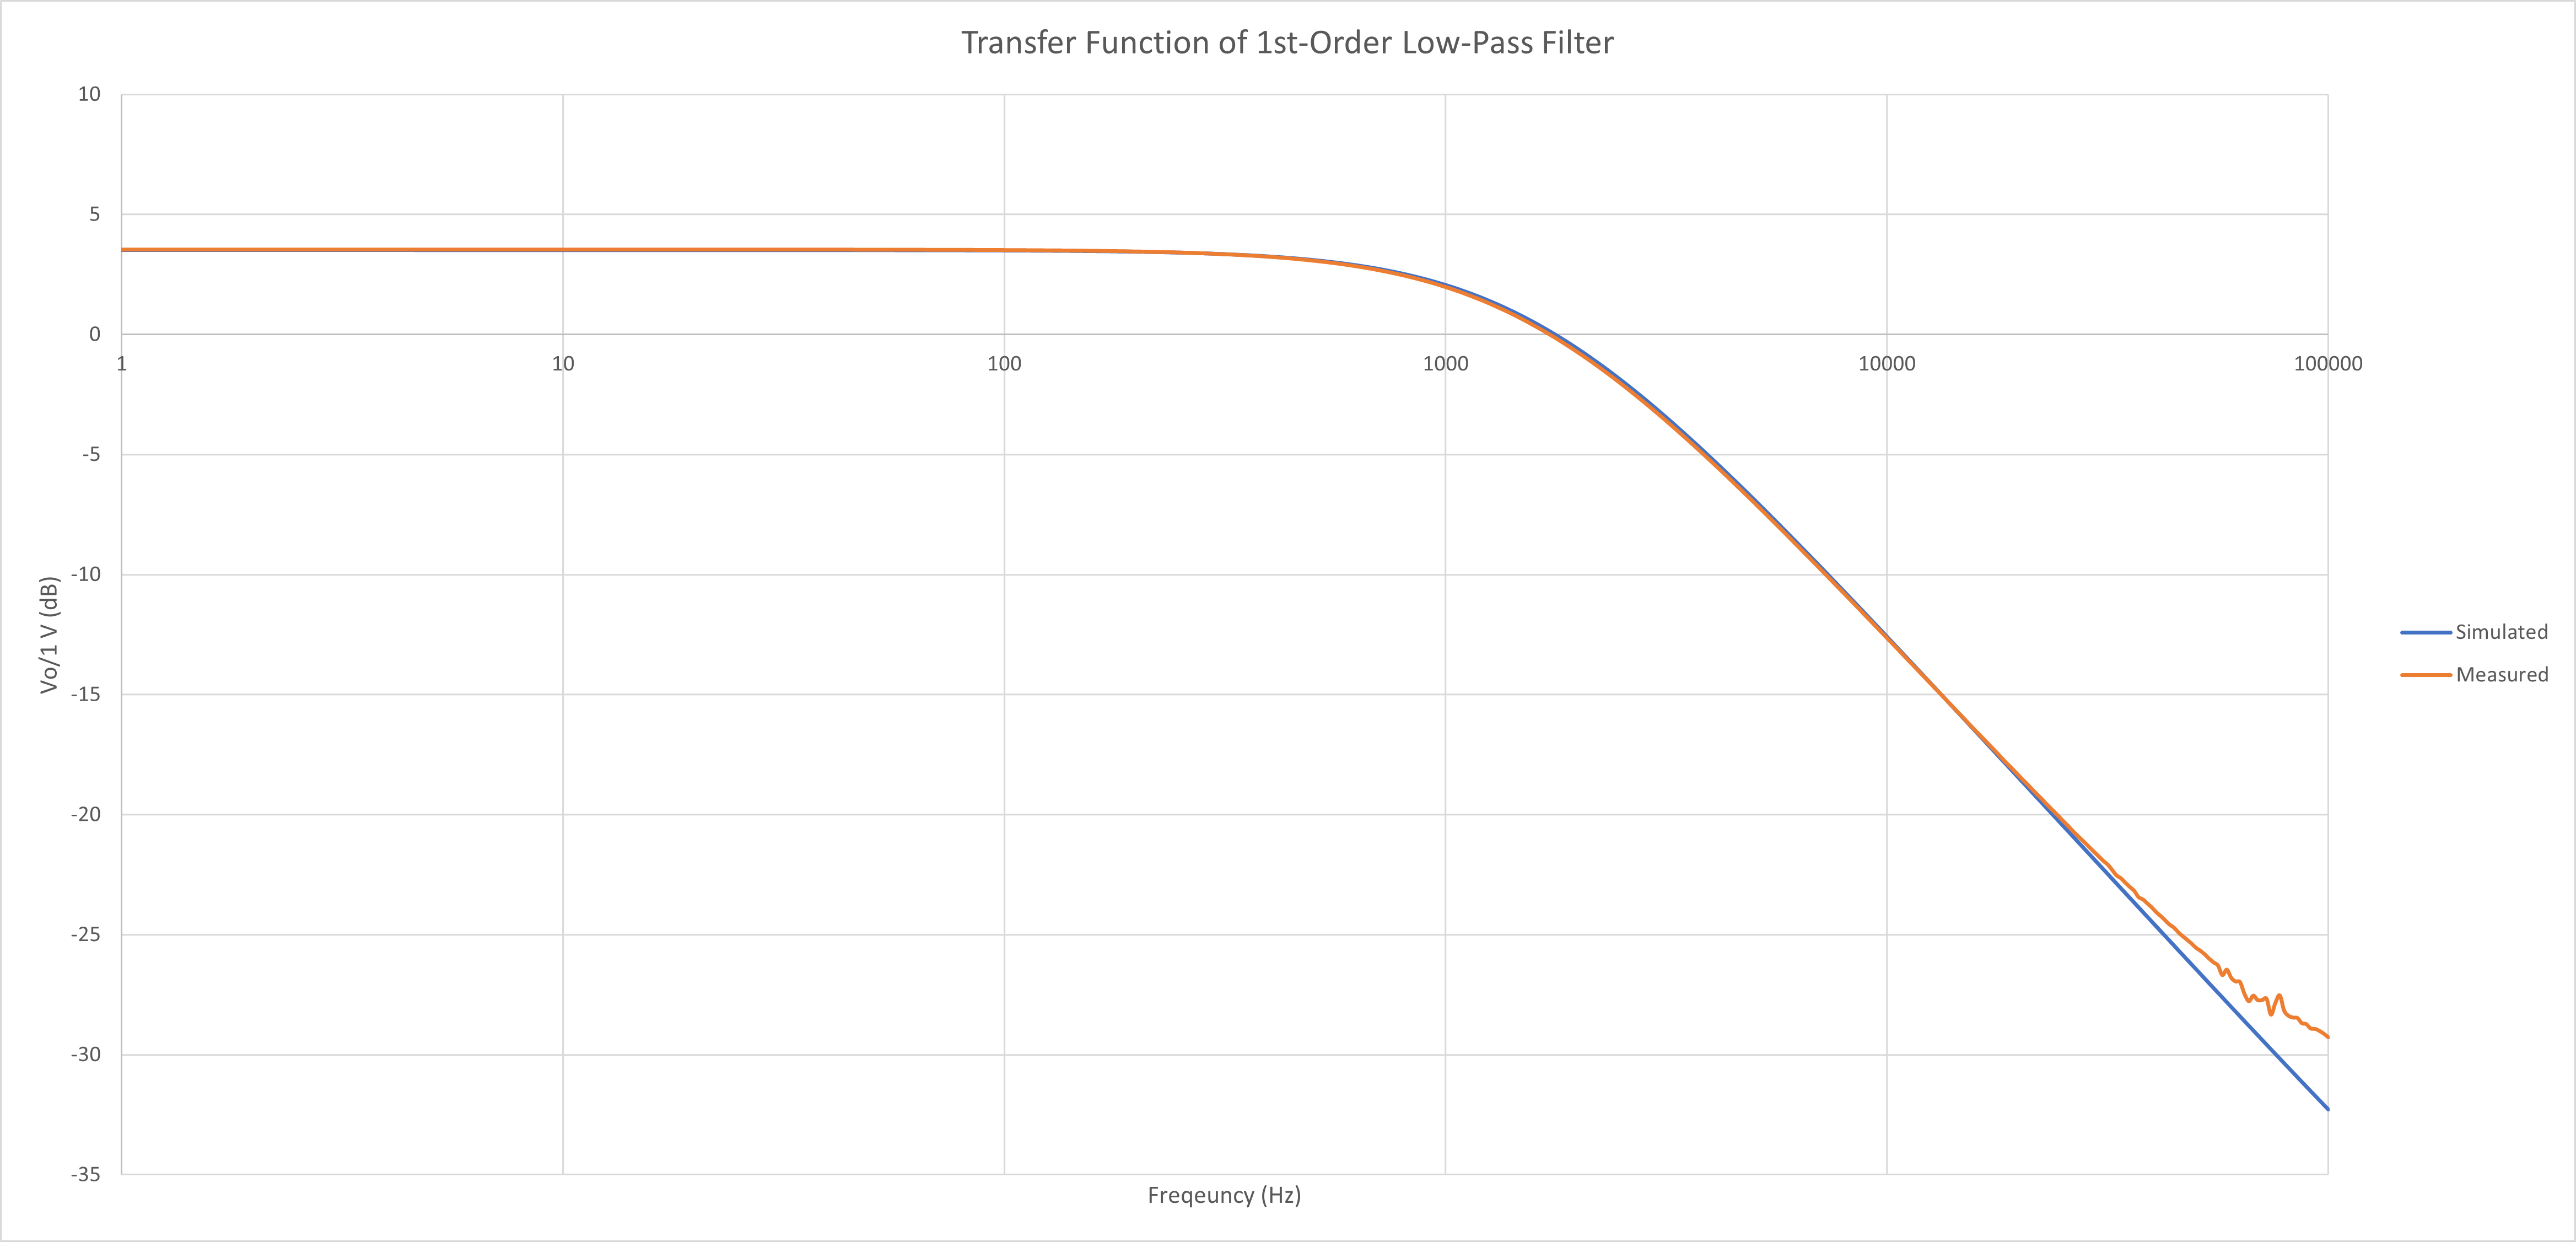
\includegraphics[width=0.95\textwidth]{Q1}
        \caption{\label{fig:Q1}Transfer Function for 1st-Order Low-Pass Filter in Part 1}
        \end{figure}
    \end{enumerate}
    \section*{Part 2}
    \item [\textbf{Q2.}]
    \begin{equation*}
    \begin{aligned}
        T(s) &= \frac{V_o(s)}{V_{in}(s)} \\
        0 &= \frac{V_1-V_{in}}{R_1}+\frac{V_1-V_o}{1/sC-1}+\frac{V_1}{R_2+1/sC_2} \\
        V_2 &= V_3 \\
        V_2 &= V_1 (\frac{1/sC_2}{R_2+1/sC_2}) = V_3 = V_o \frac{R_3}{R_3+R_4} \\
        \frac{V_o}{V_{in}} = T(s) &= \frac{R_3+R_4}{s^2(C_1C_2R_1R_2R_3) + s(C_2R_2R_3 + C_2R_1R_3 - C_1R_1R_4) + R_3} \\
        &= \frac{200 000}{s^2(0.0022) + s(34) + 100 000} \\
        &= \frac{200 000(1/0.0022)}{s^2 + s(\frac{34}{0.0022}) + 100 000(1/0.0022)} \\
        &= \frac{1}{1.1 \times 10^{-8} s^2 + 1.7 \times 10^-4 s + 0.5} \\
        Q \approx 0.436 
    \end{aligned}
    \end{equation*}
    The low-frequency gain (let $s = 0$) is equal to 2, which roughly matches the simulated low-frequency gain (6.02 dB or approximately 2 V/V) and the measured low-frequency gain (6.06 dB or approximately 2 V/V).
    \item [\textbf{Q3.}]
    The pole frequencies can be found by factoring the transfer function $T(s)$, to get $s = -11503$ or $s = -3951$. Converting this to frequency, we get $f = 1830$ Hz or $f = 629$ Hz. The $f_{max}$ is at the start (1 Hz), due to the transfer function having no zeros, and the peak value of the magnitude is the low-frequency gain.
    \begin{table}[ht]
        \centering
        \begin{tabular}{l|c|c|c|}
        \cline{2-4}
         &
          \multicolumn{1}{c|}{Calculated} &
          \multicolumn{1}{c|}{Measured} &
          Simulated \\ \hline
        \multicolumn{1}{|l|}{pole frequency $f_o$ (Hz)}      & 629 & 600 & 600  \\ \hline
        \multicolumn{1}{|l|}{cut-off frequency $f_c$ (Hz)}   & 400 & 407 & 402 \\ \hline
        \multicolumn{1}{|l|}{pole quality factor $Q$} & 0.436 & N/A & N/A \\ \hline
        \multicolumn{1}{|l|}{\begin{tabular}[c]{@{}l@{}}peak value of the magnitude\\ of the transfer function (dB)\end{tabular}} & 6
           & 6.02
           & 6.06
           \\ \hline
        \multicolumn{1}{|l|}{frequency $f_{max}$ (Hz)}           & 1 & 1 & 1 \\ \hline
        \end{tabular}
        \caption{\label{tab:Q3}Question 3}
    \end{table} \\
    The measured and simulated values generally matched the calculated values.
    \begin{figure}[ht]
        \centering
        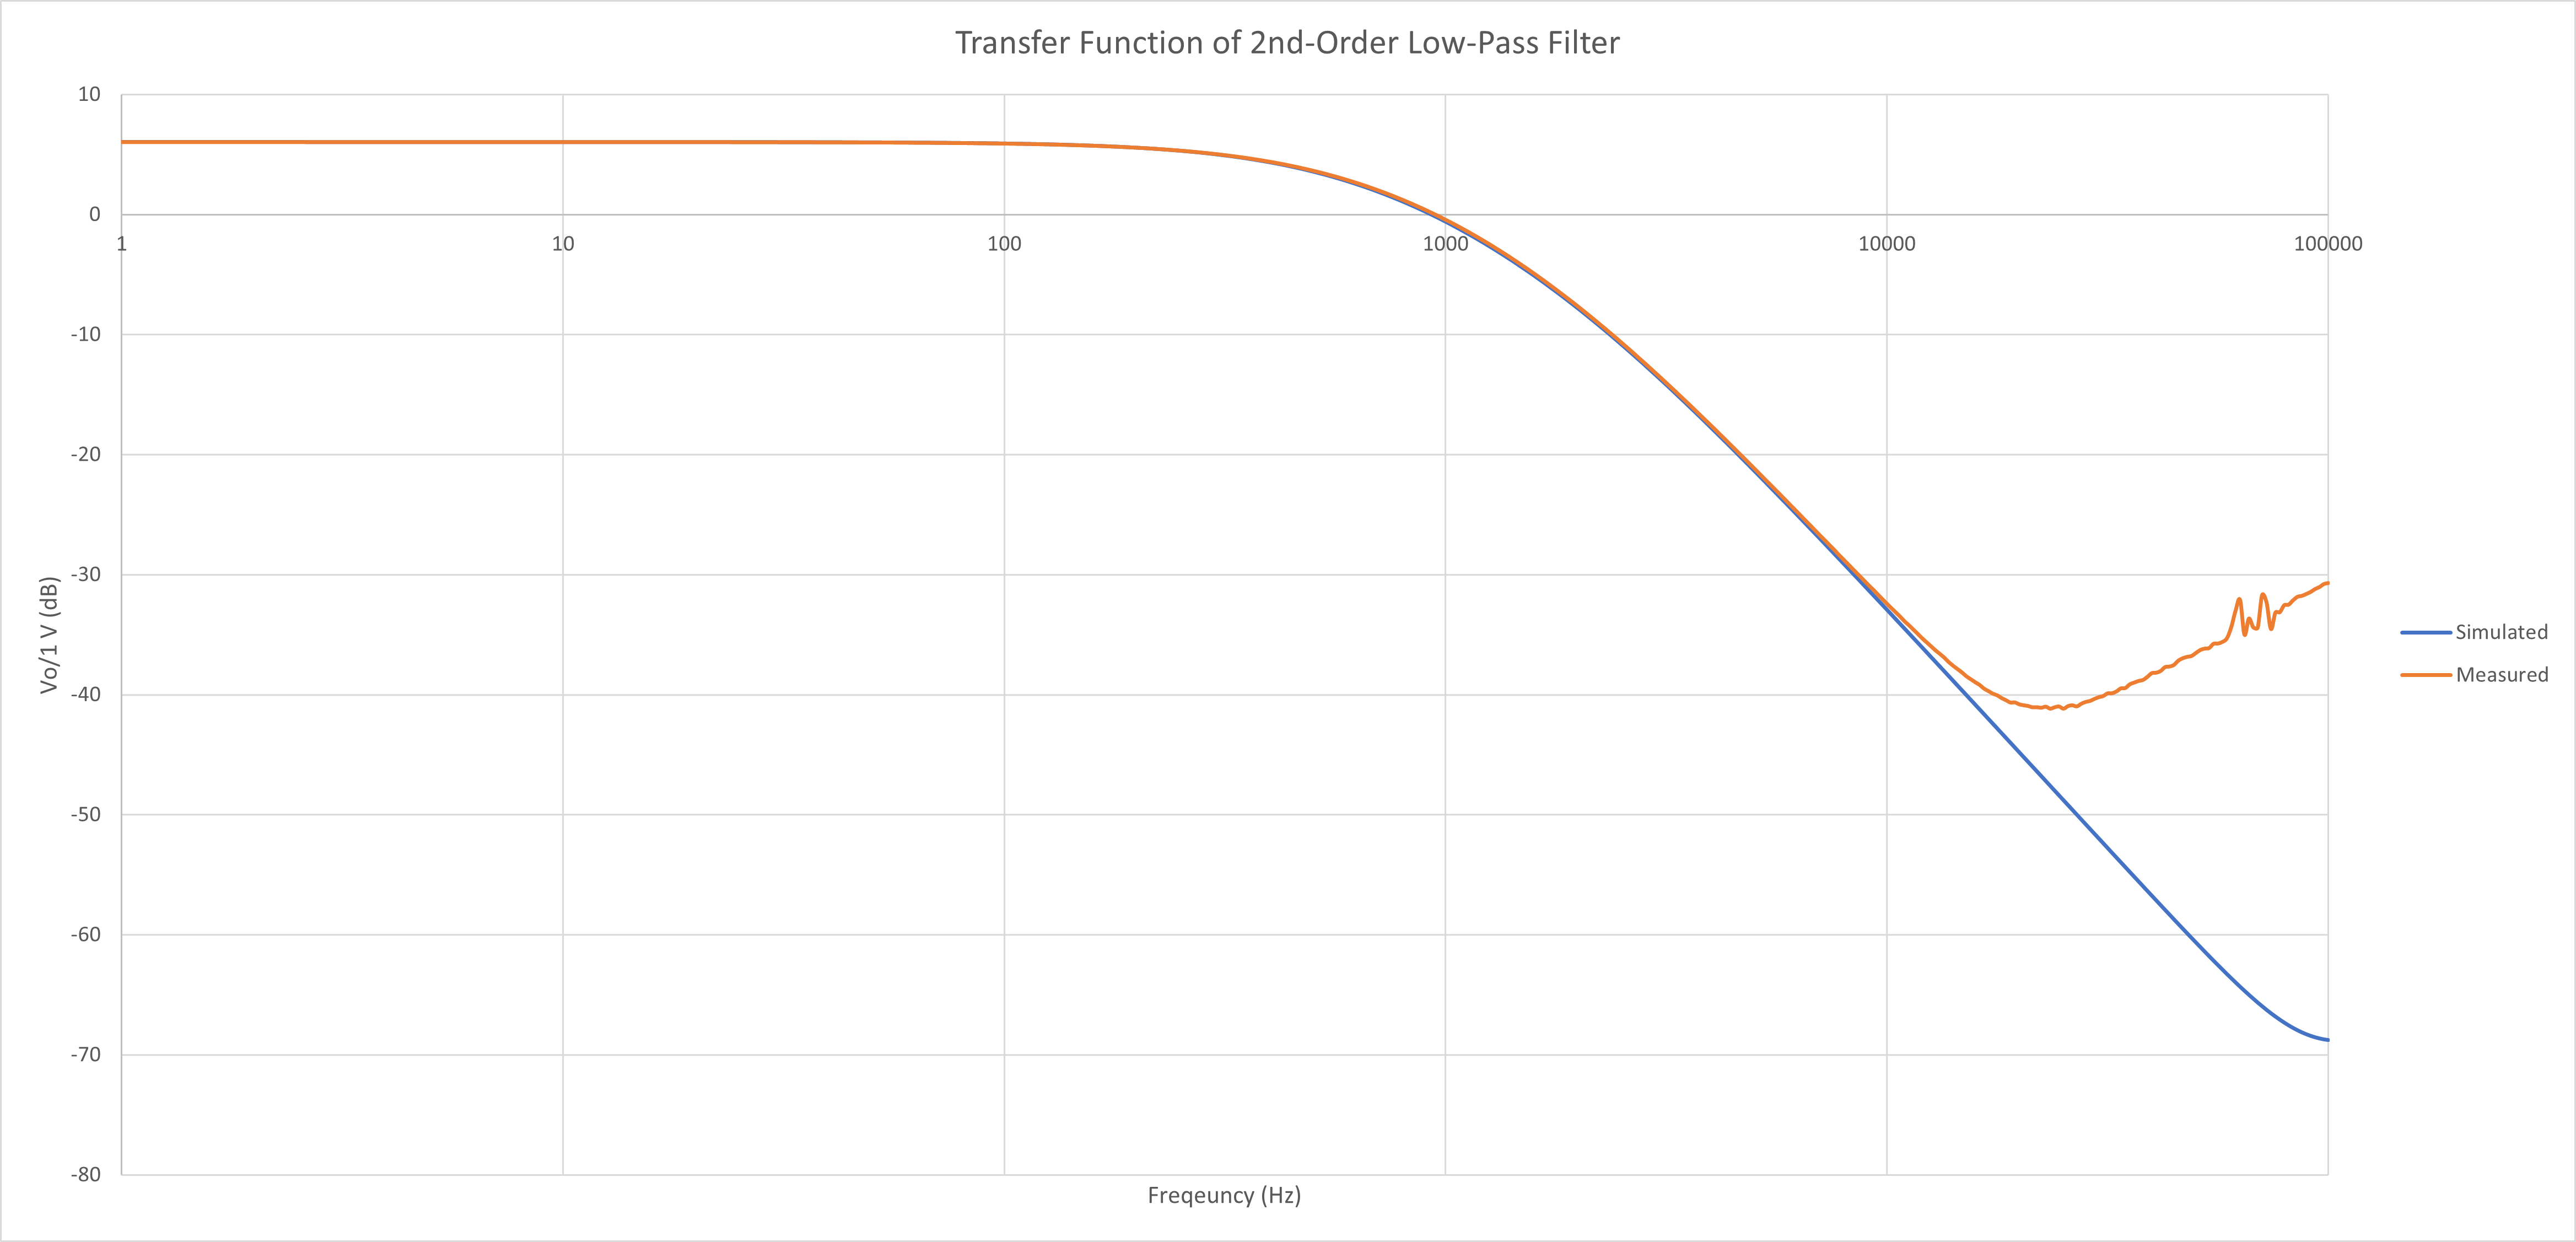
\includegraphics[width=0.95\textwidth]{Q2}
        \caption{\label{fig:Q1}Transfer Function for 2nd-Order Low-Pass Filter in Part 2}
    \end{figure} \newpage
    \section*{Part 3}
    \item [\textbf{Q4.}]
    \begin{equation*}
    \begin{aligned}
        0 &= \frac{V_1-V_{in}}{R_1} + \frac{V_1-V_o}{1/sC_1} + \frac{V_1}{1/sC_2} \\
        -\frac{V_1}{1/sC_2} &= \frac{V_o}{R_2} \\
        \frac{V_o}{V_{in}} = T(s) &= \frac{1}{-1/R_2sC_2 - \frac{C_1R_1}{C_2R_2}-R_1/R_2 - R_1sC_1}
    \end{aligned}
    \end{equation*}
    The simulated and measured center frequency gain were found by approximately -6 dB and -6.3 dB.
    \item [\textbf{Q5.}]
    The center frequency can found by :
    \begin{table}[ht]
        \centering
        \begin{tabular}{l|c|c|c|}
        \cline{2-4}
        & \multicolumn{1}{c|}{Calculated} & \multicolumn{1}{c|}{Measured} & Simulated \\ \hline
        \multicolumn{1}{|l|}{center frequency (Hz)}    &                                 & 600                              & 600           \\ \hline
        \multicolumn{1}{|l|}{pole quality factor} &                                 & N/A                            & N/A          \\ \hline
        \multicolumn{1}{|l|}{pole frequencies}    &                                 &                               &            \\ \hline
        \multicolumn{1}{|l|}{3-dB bandwidth (Hz)}      &                                 &   1292                            &    1342       \\ \hline
        \end{tabular}
        \end{table}
    \begin{figure}[ht]
        \centering
        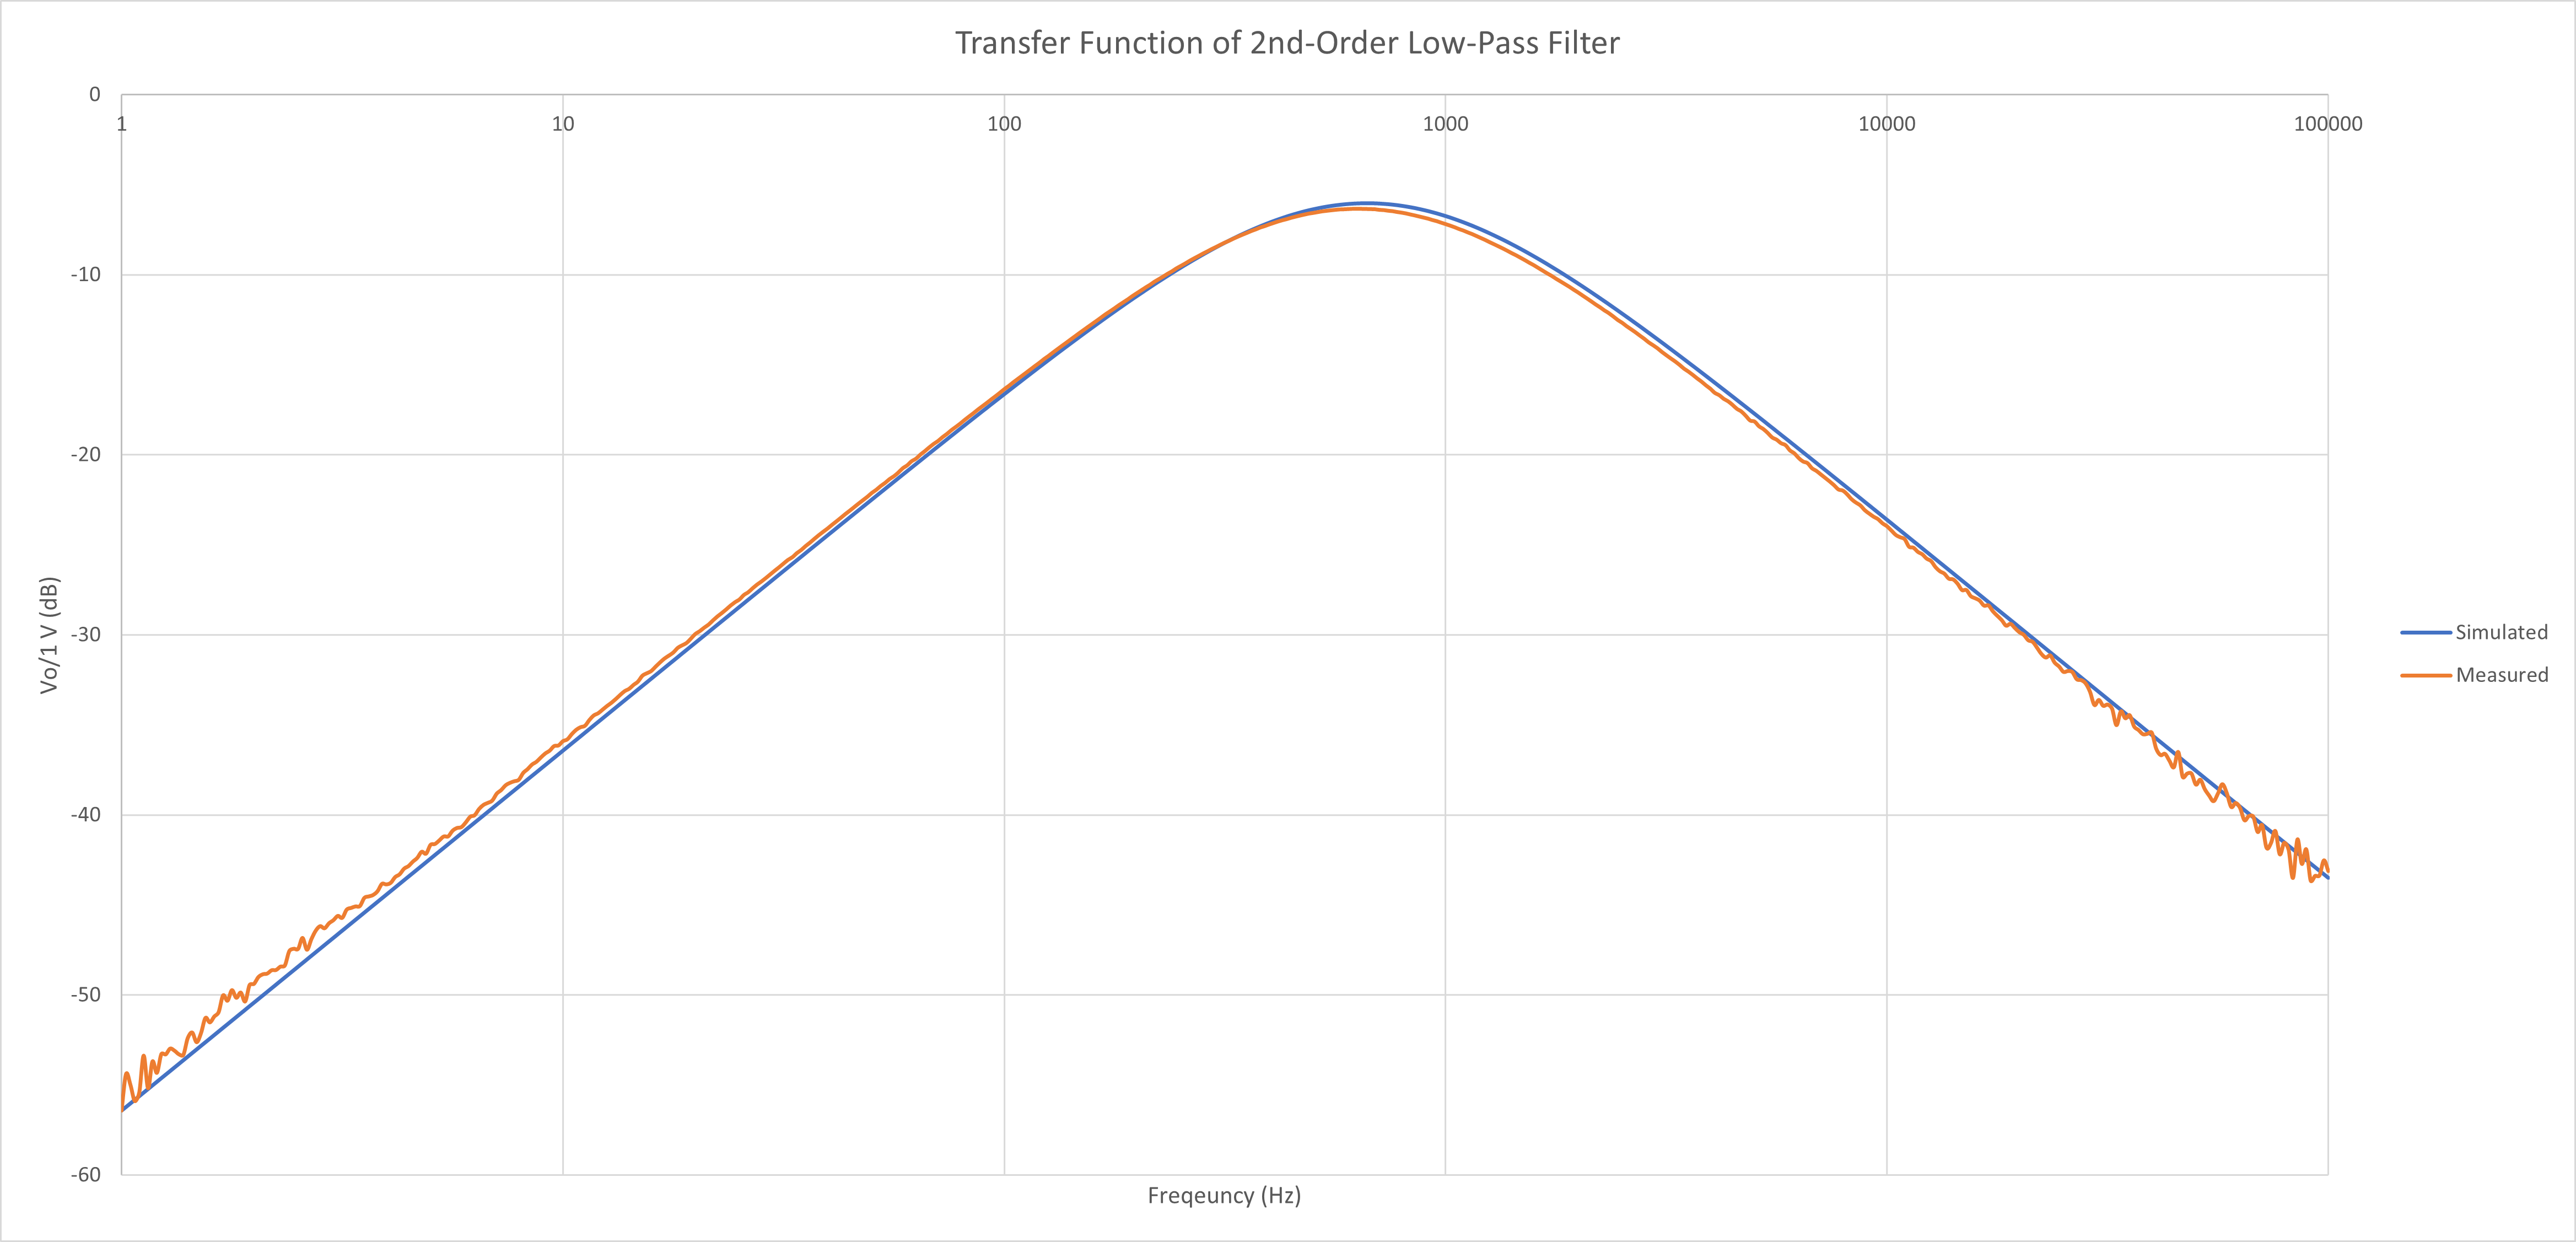
\includegraphics[width=0.95\textwidth]{Q3}
        \caption{\label{fig:Q1}Transfer Function for 2nd-Order Band-Pass Filter in Part 3}
    \end{figure} \newpage
\end{itemize}
\end{document}